\documentclass[12pt]{article}
\usepackage{amsmath,amsfonts,bbm,xfrac}
\usepackage{fancyhdr,enumitem,xcolor,placeins,subcaption,hyperref}
\usepackage{graphicx} % Allows including images
\usepackage[left=2.5cm, right=2.5cm, top =3cm, bottom = 3cm]{geometry}
\hypersetup{
    colorlinks=true,
    linkcolor=blue,
    filecolor=blue,      
    urlcolor=blue,
    }	
\setcounter{MaxMatrixCols}{10}
	
	
	
\pagestyle{plain}
\pagestyle{fancy} 
\rhead{Winter 2023} 
\chead{} 
\lhead{ECON 33530 - Firm Dynamics and Economic Growth} 
\lfoot{} 
\cfoot{} 
\rfoot{\thepage} 
\renewcommand{\headrulewidth}{0.5pt} 
\renewcommand{\footrulewidth}{0pt} 

\title{Firm Dynamics and Economic Growth \\ \large{Problem Set I}}
\author{Jose M. Quintero\thanks{Full replication code can be found at \url{https://github.com/jmquintero925/FD-EG-Ufuk}}}
\date{ }

\begin{document}

\maketitle

In this assignment you will replicate some of the key empirical findings of Akcigit and Kerr (2018) published version, from now on referred to as AK. There will be one important difference in the sample used for the analysis: while AK uses firm data from the Census, which is not publicly available, you will use a database of publicly traded firms, Compustat.

Your assignment is to replicate figures 1 and 2 from AK. Below are some guidelines for the assignment. NOTE: not all of the steps required to replicate the findings are listed below. You need to take some extra steps, which you will need to figure out yourself.

Optional: if you want to have more fun, you can look at the working paper version (NBER Working Paper \#16443), which contains many additional empirical facts, and try to replicate any of them.

\section{Download Data.}

\begin{enumerate}[leftmargin=0pt, label=\textbf{(\alph*)}]

\item Get an account on WRDS \\  (\url{https://wrds-www.wharton.upenn.edu) in order to access Compustat.}

\item Access Compustat - Capital IQ - North America. Select the monthly-updated Fundamental Annual Database.

\item Download the variables you need. Hints: select a date range that looks reasonable to you. Choose "gvkey" for company code. Select "Search the Entire Database". Select "EXCH" and "FIC". Select the variables "EMP", "SALE", "XRD", "SIC" in the query.

\item You will also need patent data and you will need to match patents to their assignee firms in Compustat. The NBER provides a USPTO patent database, as well as a firm identifier already matched to Compustat. You can access patents, citations and Compustat merge identifier at \url{https://sites.google.com/site/patentdataproject/}.

\end{enumerate}

\section{Preliminary analysis.}

\begin{enumerate}[leftmargin=0pt, label=\textbf{(\alph*)}]

\item Sample Selection. Keep only firms incorporated in the US (hint: use "FIC") and firms that do business in U.S. dollars (hint: use "CAD").

\item Merge your Compustat sample with the patent database. To limit issues of truncation, limit your analysis to the year 1980-2000, i.e. only consider patents applied for ("appyear") between 1980-2000. What are the issues related to truncation when it comes to patents?
\item[\textbf{(S)}] Truncation creates is that patent application is a proxy for innovation flow. Thus trucating within a period will create noise around the innovation flow, favoring firms that applied to patents during the period of interest. 

\item Provide a table of summary statics (this will have to include some of the variables that you will compute in the next steps).
\item[\textbf{(S)}] The statistics for the full sample is presented in Table \ref{tab:ss_full_sample}
\begin{table}[htb]
\caption{Summary Statistics}
\label{tab:ss_full_sample}
\begin{center}
\begin{tabular}{lcccccc}
\hline\hline \noalign{\smallskip}Variable & Obs. & Mean & Std. Dev. & Min & Median & Max\\\hline
\noalign{\smallskip}\noalign{\smallskip}Employment & 142,488 & 5.041 & 23.308 & 0.000 & 0.478 & 1,244\\
 Sales & 160,228 & 748.285 & 3,828.534 & -80.817 & 54.635 & 206,083\\
R\&D & 73,230 & 23.926 & 188.644 & -0.397 & 0.866 & 8,900\\
Innovative & 184,206 & 0.299 & 0.458 & 0 & 0 & 1\\
\noalign{\smallskip}\hline\hline
\end{tabular}
\end{center}

\scriptsize{\textbf{Notes:} Innovative is a dummy variable that takes the value of 1 whenever the firm has at least one patent during the period of interest. }
\end{table}
\FloatBarrier

\item What is the share of firms which have at least one patent? We will refer to the firms with at least one patent as "innovative firms".
\item[\textbf{(S)}] As seen in Table \ref{tab:ss_full_sample} the share of innovative firms is close to 30\% of the sample. 

\item Compare your sample of innovative firms to the population of Compustat firms. How do they differ? Think of a way to illustrate the differences (hint: for example, differences in employment size).
\item[\textbf{(S)}] The descriptive statistics controlling by the variable indicating if the firm has a patent during the period of interest is presented in Table \ref{tab:ss_by_inn}
\begin{table}[htb]
\caption{Summary Statistics}
\label{tab:ss_by_inn}
\vspace*{-10pt}
\begin{center}
\resizebox{\textwidth}{!}{
\begin{tabular}{l|ccc|ccc|cc}
\hline\hline \noalign{\smallskip} & \multicolumn{3}{c}{Not Innovative} & \multicolumn{3}{c}{Innovative} &  & \\ \hline
 & Obs & Mean & Std. Dev. & Obs & Mean & Std. Dev. & $\mu_1-\mu_0$ & $ p$-value\\
\noalign{\smallskip}\hline \noalign{\smallskip}Employment & 93,126 & 3.161 & 12.272 & 49,362 & 8.586 & 35.565 & 5.425$^{***}$ & 0.00\\
Sales & 107,863 & 453.263 & 1,950.590 & 52,365 & 1,355.978 & 6,038.598 & 902.715$^{***}$ & 0.00\\
R\&D & 36,334 & 3.203 & 27.731 & 36,896 & 44.334 & 262.745 & 41.131$^{***}$ & 0.00\\
\noalign{\smallskip}\hline\hline
\end{tabular}
}
\end{center}

\scriptsize{\textbf{Notes:} $^{***}$ denotes that the mean difference is statistically significant different than 0 at the 99\% . }
\end{table}
From Table \ref{tab:ss_by_inn} we see that there are significant differences between innovative firms and non-innovative firms. On average
\item From now on, focus your analysis on the sample of innovative firms. 

\end{enumerate}

\FloatBarrier
\section{Firm Growth by Firm Size. (Figure 1).}

\begin{enumerate}[leftmargin=0pt, label=\textbf{(\alph*)}]

\item Build the main variable of employment growth used in the paper, i.e.

$E m p G r_{f, t}=\left(E m p_{f,+1 t}-E m p_{f, t}\right) / E m p_{f, t}$. Apply the same winsorization discussed in the paper.

\item Replicate Figure 1 and the corresponding regression. On the x-axis, you will use $E m p_{f, t}$. On the y-axis, you will use $E m p G r_{f, t}$. Hint: you can use the command binscatter.
\item[\textbf{(S)}] The replicated Figure is presented in Figure \ref{fig:growth_firm_size_1}. Just as in Akcigit and Kerr (2018) there is an negative relation between firm growth in terms of employees and their current employment. 
\begin{figure}[htb]
\caption{Employment Growth by Firm Size}
\label{fig:growth_firm_size}
\centering
     \begin{subfigure}[b]{0.48\textwidth}
         \centering
         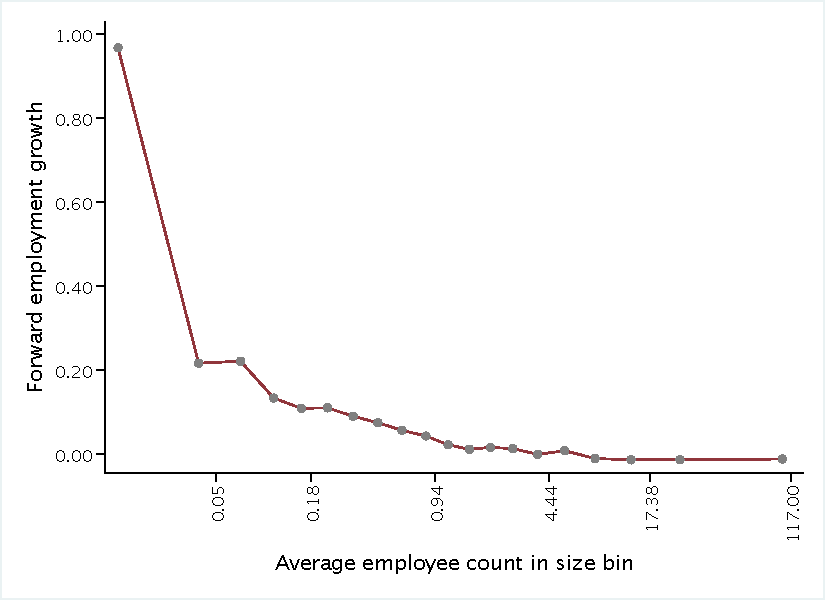
\includegraphics[width=\textwidth]{Figures/Figure1b.pdf}
         \caption{Percentage Growth}
         \label{fig:growth_firm_size_1}
     \end{subfigure}
     \hfill
     \begin{subfigure}[b]{0.48\textwidth}
         \centering
         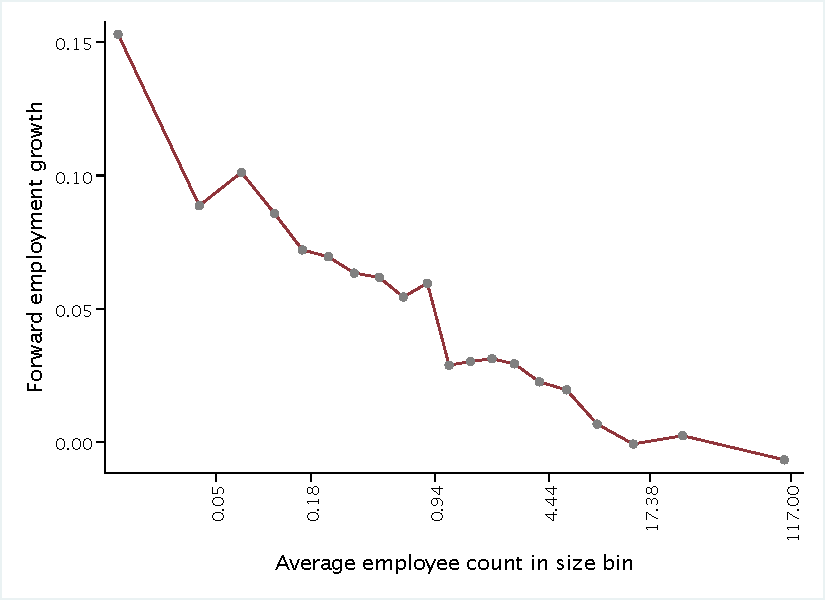
\includegraphics[width=\textwidth]{Figures/Figure1c.pdf}
         \caption{DHS Growth}
         \label{fig:growth_firm_size_2}
     \end{subfigure}
\end{figure}


The regression corresponding to this exercise is presented in Table \ref{tab:reg1}. Just like in the AK paper, there is a significant negative relation between employment and and firm growth. Specifically, an increase in one percent of the firm will decrease their growth by 0.08\%. 

\begin{table}[htb]
\centering
\caption{Firm Growth and Employment}
\label{tab:reg1}
\documentclass[]{article}
\setlength{\pdfpagewidth}{8.5in} \setlength{\pdfpageheight}{11in}
\begin{document}
\begin{tabular}{lc} \hline
 & (1) \\
VARIABLES & empgr \\ \hline
 &  \\
log\_emp & -0.0833*** \\
 & (0.0146) \\
 &  \\
Observations & 46,295 \\
 R-squared & 0.0169 \\ \hline
\multicolumn{2}{c}{ Robust standard errors in parentheses} \\
\multicolumn{2}{c}{ *** p$<$0.01, ** p$<$0.05, * p$<$0.1} \\
\end{tabular}
\end{document}

\end{table}

\item Replicate your graph for the alternative measure of firm growth rate cited in the paper, i.e. $E m p G r_{f, t}=\left(E m p_{f,+1 t}-E m p_{f, t}\right) /\left(0.5\left(E m p_{f,+1 t}+E m p_{f, t}\right)\right)$.

\item[\textbf{(S)}] The results using the Davis, Haltinwanger and Schun measure for growth are presented in Figure \ref{fig:growth_firm_size_2}. Note that the relation is still the same but the scale is significantly different. The reason behind this change is that the DHS measure is absolutely bounded by 2 and thus the outlines will have a less meaningful impact. 

\end{enumerate}


\FloatBarrier
\section{Innovation Intensity by Firm Size. (Figure 2).}

\begin{enumerate}[leftmargin=0pt, label=\textbf{(\alph*)}]


\item Compute the number of patents per employment (i.e. total number of patents applied for in a given year by a firm, divided by employment). How lumpy is patenting in your dataset? Decide whether to apply the same five-year windows discussed in the paper and explain why.
\item[\textbf{(S)}] After inspection patenting is still lumpy. Conditional on the innovative sample, the median number of patents filed by a firm in a given year is 0. Moreover, on average, firms file for a new patent once every 1.5 years. Thus, I used a 5-year window as in the AK paper to smooth out this lumpiness. 

\item Replicate Figure 2 and the corresponding regression.
\item[\textbf{(S)}] The results are presented in Figure \ref{fig:patent_intesity}. As previously mentioned, I use windows of 5 years and include the 2000s in the last window. 

\begin{figure}[htb]
         \centering
         \caption{Patent Intensity and Firm Size}
         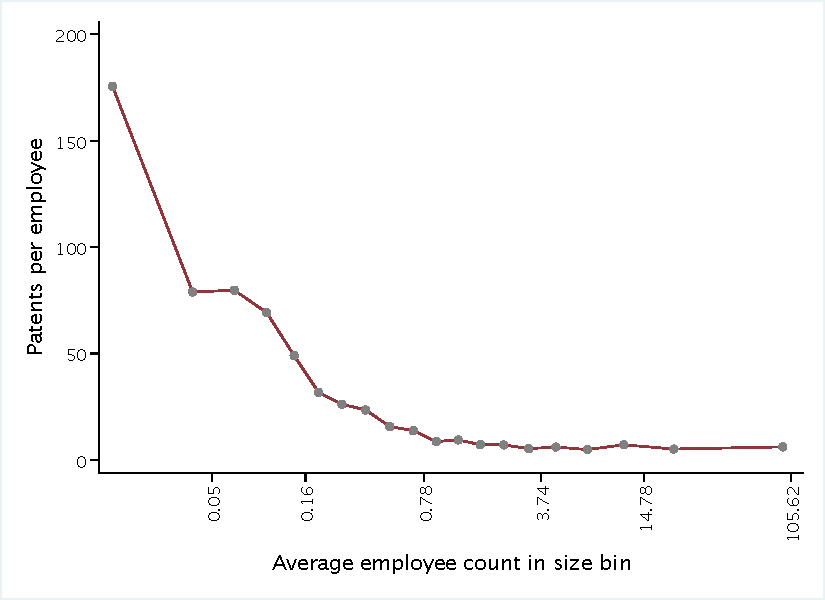
\includegraphics[width=0.45\textwidth]{Figures/Figure4b.pdf}
         \label{fig:patent_intesity}
\end{figure}

As in the AK paper, small firms are more intense in patenting activity. The regression is presented in Table \ref{tab:reg2}. 

\begin{table}[htb]
\centering
\caption{Firm Growth and Employment}
\label{tab:reg2}
\small{
\begin{tabular}{lc} \hline\hline
Variable & $\sfrac{\text{Patents}_{ft}}{\text{Empt}_{ft}}$ \\ \hline
$\log\left(\text{Emp}_{ft}\right)$ & -0.1187*** \\
 & (0.0090) \\
\hline
Observations & 11,483 \\
 R-squared & 0.1457 \\ \hline\hline
\multicolumn{2}{l}{ Robust standard errors in parentheses} \\
\multicolumn{2}{l}{ *** p$<$0.01, ** p$<$0.05, * p$<$0.1} \\
\end{tabular}
}
\end{table}

Again, I find a robust negative correlation suggesting that small firms are more intense in their patenting activity. 
\end{enumerate}


\FloatBarrier
\section{R\&D Intensity by Firm Size.}

\begin{enumerate}[leftmargin=0pt, label=\textbf{(\alph*)}]

\item In class, we discussed how the relationship between $R \& D$ intensity and firm size has evolved over time. We will replicate this finding here.

\item Run a regression of $\log \mathrm{R} \& \mathrm{D}$ expenditure over log sales in each year, with industry fixed effects :

\begin{equation*}
\ln \left(R \& D_{i, j, t}\right)=\beta_{0}+\beta_{1} \ln \left(\text { Sales }_{i, j, t-1}\right)+\delta_{j}+\epsilon_{i, j, t}
\end{equation*}

where $i$ indicates a firm, $j$ a sector and $t$ a year. $\delta_{j}$ are sector fixed-effects. Your coefficient of interest is $\beta_{1}$. You will obtain a different coefficient $\beta_{1}$ for every year in your sample. Plot the coefficients you obtain over time, including the standard errors. Hint: You will have years on the $\mathrm{x}$-axis and $\beta_{1}$ on the $\mathrm{y}$-axis.
\item[\textbf{(S)}] The results for each regression are presented in Figure \ref{fig:rd_time}. 

\begin{figure}[htb]
         \centering
         \caption{R\&D and Sales}
         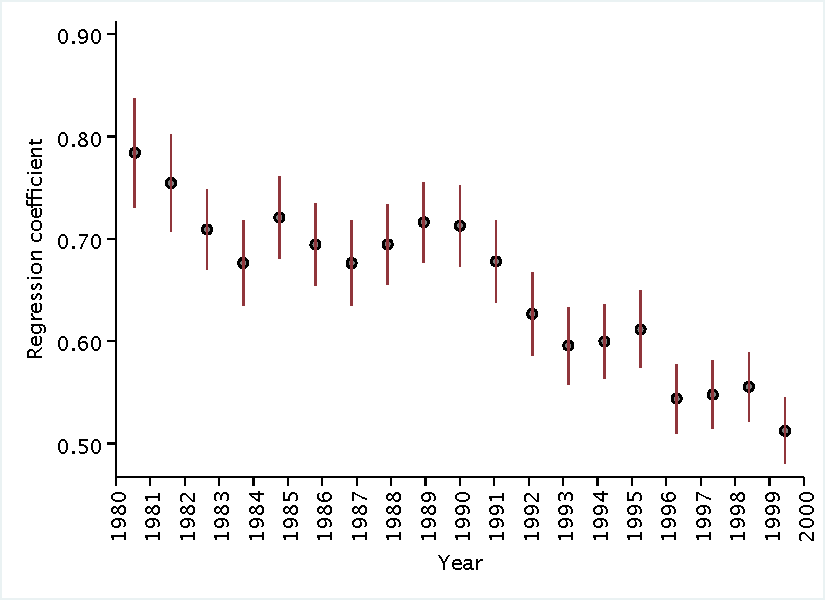
\includegraphics[width=0.5\textwidth]{Figures/Figure5b.pdf}
         \label{fig:rd_time}
\end{figure}

\item How did the relationship between R\&D intensity and firm size evolve over time? Explain.
\item[\textbf{(S)}] Over time, the relationship between sales and R\&D has decrease although it has always been statistically significant. It is worth highlighting, during the second half of 1980s, the effect was relatively stable. 
\end{enumerate}

\FloatBarrier

\section{Discussion}

\begin{enumerate}[leftmargin=0pt, label=\textbf{(\alph*)}]

\item How do your results compare to the findings in the paper? Explain why.
\item[\textbf{(S)}] Overall, the results are consistent with the findings of Akcigit and Kerr (2018). Figure \ref{fig:growth_firm_size_1} and \ref{fig:patent_intesity} replicate the results qualitatively. Similarly, the signs of regressions \ref{tab:reg1} and \ref{tab:reg2} are consistent with the  results of the original paper. The difference in magnitudes is due to sample selection as firms showing up in Compustat are publicly traded companies. 

\item Do you believe that there are limitations in using Compustat versus Census data for the analysis? If so, what type of limitations?
\item[\textbf{(S)}] There is a significant bias in using Compustat versus the Census data. There is a considerable bias selection on publicly traded firms versus the entire universe of firms. Of course, firms that can innovate represent another margin of choice, which could be correlated with being a public company. Nevertheless, firms in Compustat are on average older, bigger and more capital/skill intensive. All these traits interact with incentives/ability to innovate and thus one has to account for these bias when restricting to Compustat.  

\item What do these findings imply? How are they useful to learn something about firm dynamics and innovation? How could you use them to inform a theoretical model?
\item[\textbf{(S)}] These results are particularly relevant as they marka departure from the stylized facts presented in Klette and Kortum (2004). For instance, in their model, patent intensity is constant across firm size. These fact is particularly relevant, as it highlights how as firms grow, their innovation incentives change. 

Thus, as done by Akcigit and Kerr (2018), these moment can identify parameters of structural model and help design better industrial policy. To do so, these stylized facts create a mind teaser for the possible mechanism that might be acting and generating these results. 

\end{enumerate}
\end{document}